\documentclass[11pt]{article}

\usepackage{times}
\usepackage{epsf}
\usepackage{epsfig}
\usepackage{amsmath, alltt, amssymb, xspace}
\usepackage{wrapfig}
\usepackage{fancyhdr}
\usepackage{url}
\usepackage{verbatim}
\usepackage{fancyvrb}
\usepackage{float}

\usepackage{subfigure}
\usepackage{cite}
\usepackage{hyperref}
\hypersetup{%
    pdfborder = {0 0 0}
}
\topmargin      -0.50in  % distance to headers
\oddsidemargin  0.0in
\evensidemargin 0.0in
\textwidth      6.5in
\textheight     8.9in 


%\centerfigcaptionstrue

%\def\baselinestretch{0.95}


\newcommand\discuss[1]{\{\textbf{Discuss:} \textit{#1}\}}
%\newcommand\todo[1]{\vspace{0.1in}\{\textbf{Todo:} \textit{#1}\}\vspace{0.1in}}
\newtheorem{problem}{Problem}[section]
%\newtheorem{theorem}{Theorem}
%\newtheorem{fact}{Fact}
\newtheorem{define}{Definition}[section]
%\newtheorem{analysis}{Analysis}
\newcommand\vspacenoindent{\vspace{0.1in} \noindent}

%\newenvironment{proof}{\noindent {\bf Proof}.}{\hspace*{\fill}~\mbox{\rule[0pt]{1.3ex}{1.3ex}}}
%\newcommand\todo[1]{\vspace{0.1in}\{\textbf{Todo:} \textit{#1}\}\vspace{0.1in}}

%\newcommand\reducespace{\vspace{-0.1in}}
% reduce the space between lines
%\def\baselinestretch{0.95}

\newcommand{\fixmefn}[1]{ \footnote{\sf\ \ \fbox{FIXME} #1} }
\newcommand{\todo}[1]{
\vspace{0.1in}
\fbox{\parbox{6in}{TODO: #1}}
\vspace{0.1in}
}

\newcommand{\mybox}[1]{
\vspace{0.2in}
\noindent
\fbox{\parbox{6.5in}{#1}}
\vspace{0.1in}
}


\newcounter{question}
\setcounter{question}{1}

\newcommand{\myquestion} {{\vspace{0.1in} \noindent \bf Question \arabic{question}:} \addtocounter{question}{1} \,}

\newcommand{\myproblem} {{\noindent \bf Problem \arabic{question}:} \addtocounter{question}{1} \,}



\newcommand{\copyrightnotice}[1]{
\vspace{0.1in}
\fbox{\parbox{6in}{
      This lab was developed for the Labtainer framework by the Naval Postgraduate 
      School, Center for Cybersecurity and Cyber Operations.
      This work is in the public domain, and cannot be copyrighted.}}
\vspace{0.1in}
}


\newcommand{\idea}[1]{
\vspace{0.1in}
{\sf IDEA:\ \ \fbox{\parbox{5in}{#1}}}
\vspace{0.1in}
}

\newcommand{\questionblock}[1]{
\vspace{0.1in}
\fbox{\parbox{6in}{#1}}
\vspace{0.1in}
}


\newcommand{\argmax}[1]{
\begin{minipage}[t]{1.25cm}\parskip-1ex\begin{center}
argmax
#1
\end{center}\end{minipage}
\;
}

\newcommand{\bm}{\boldmath}
\newcommand  {\bx}    {\mbox{\boldmath $x$}}
\newcommand  {\by}    {\mbox{\boldmath $y$}}
\newcommand  {\br}    {\mbox{\boldmath $r$}}


\newcommand{\tstamp}{\today}   
%\rfoot[\fancyplain{\tstamp} {\tstamp}]  {\fancyplain{}{}}

\pagestyle{fancy}
\lhead{\bfseries Labtainers}
\chead{}
\rhead{\small \thepage}
\lfoot{}
\cfoot{}
\rfoot{}




\begin{document}

\begin{center}
{\LARGE Routing Basics}
\vspace{0.1in}\\
\end{center}

\copyrightnotice

\section{Overview}
This exercise explores basic network routing concepts 
in a Linux environment.  These include use of the \texttt{route}
command, defining a DNS server in the /etc/resolv.conf file,
and using Network Address Translation (NAT). 

This exercise, (and manual), is not intended to replace instruction
or independent reading on the topic of network routing and
routing in Linux systems. The exercise is intended to provide
students with an environment with which they can experiment
with the mechanics of routing network traffic.


\section{Lab Environment}
This lab runs in the Labtainer framework,
available at http://my.nps.edu/web/c3o/labtainers.
That site includes links to a pre-built virtual machine
that has Labtainers installed, however Labtainers can
be run on any Linux host that supports Docker containers.

From your labtainer-student directory start the lab using:
\begin{verbatim}
    labtainer routing-basics
\end{verbatim}
\noindent A link to this lab manual will be displayed.  

\section{Network Configuration}
This lab includes four networked computers as shown in Figure~\ref{fig:topology}.
When the lab starts, you will get four virtual terminals, one connected to each
component.
The gateway is configured to perform routing between LAN1 and LAN2, and to
route external addresses to an external gateway, e.g., to reach the Internet.
The ws1 and ws2 workstations are pre-configured to route traffic to the gateway
component.  The ws3 workstation is not yet configured for routing.

The gateway is configured to use NAT to translate
sources addresses of traffic from internal IP addresses, e.g., 192.168.1.1, to
our external address, i.e., 203.0.113.10.

\begin{figure}[htb]
\begin{center}
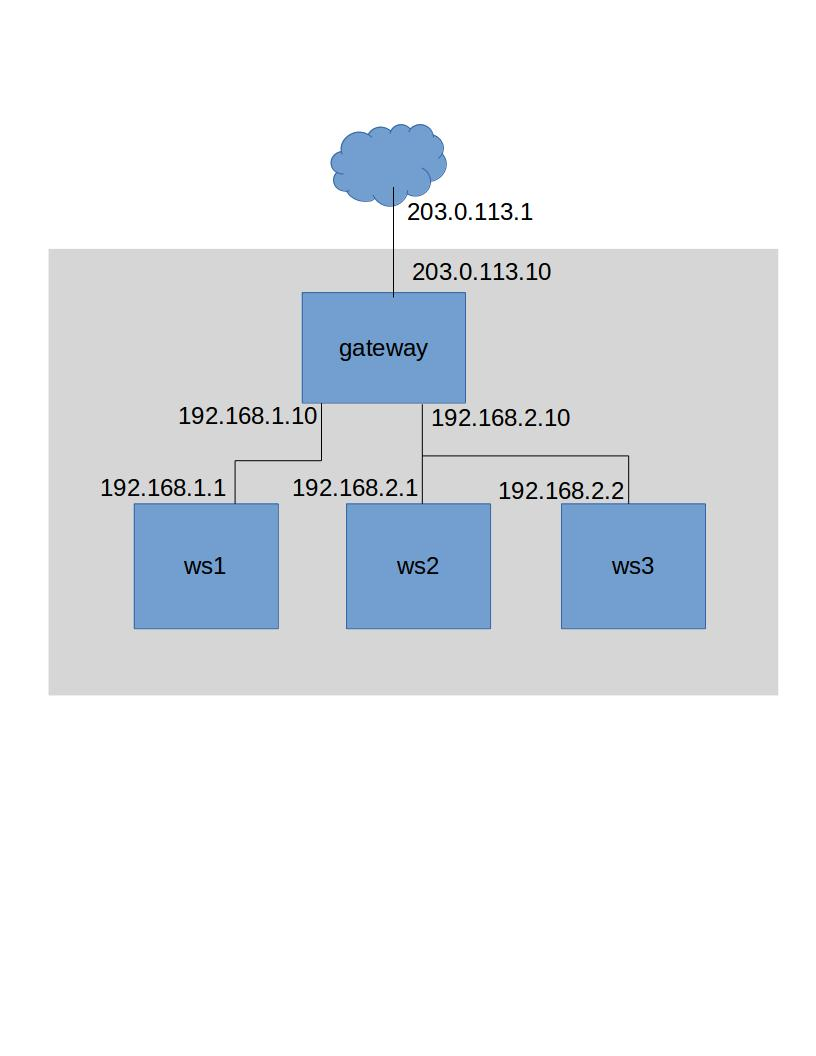
\includegraphics [width=0.8\textwidth,natwidth=621,natheight=403]{routing-basics.jpg}
\end{center}
\caption{Network topology for routing-basics lab}
\label{fig:topology}
\end{figure}

\section{Lab Tasks}
\subsection{Internal Routing}
From each of the three workstations, enter the following command:
\begin{verbatim}
    route -n
\end{verbatim}
\noindent Note how ws1 and ws2 include routing table entries that name the
gateway as the \textit{default gateway}.  This allows ws1 and ws2 to address each other, which 
can be demonstrated by using \texttt{ping} from ws1 to reach ws2:

\begin{verbatim}
    ping [ws2 IP]
\end{verbatim}

Now consider ws2 and ws3.  Since they are both on the same LAN, they can ping
each other.  Try that for yourself.  Then try to ping ws1 from ws3.  That will
fail because ws3 has no routing table entry defining what to do with traffic 
that is not destined for a LAN directly connected to ws3.

On ws3, define the gateway component as the \textit{default gateway} using the 
\texttt{route} command, but this time using \texttt{sudo} because we are altering the routing:

\begin{verbatim}
    sudo route add default gw [gateway IP]
\end{verbatim}
\noindent Then try to ping between ws1 and ws3. 

\subsection{Routing to the Internet}
The gateway component is configured to route to a simulated ISP at 203.0.113.1, which 
is a hidden component that provides routing to the Internet for this lab.  From ws2, 
try to ping www.google.com.  Then do the same from ws3.  The problem with ws3 is that
it has no domain name service (DNS) definition.  Note, routing from ws3 to the Internet
works fine, which you can confirm by pinging the IP address of www.google.com (as displayed
when you pinged from ws2).  The ws3 component simply lacks a DNS definition. 
On ws2, the DNS is defined to be the
gateway component, and this is achieved in the \texttt{/etc/resolv.conf} file \footnote{
Many Linux systems include tools for defining your DNS, and these tools will overwrite
the resolv.conf file.  That is not an issue in these labs}.  If you 
modify that file on ws3 to match that of ws2, that will tell ws3 to use the gateway
as its DNS.

\subsection{Use of Network Address Translation (NAT)}
Finally, review how the gateway component implements NAT using the \texttt{iptables} 
utility.  Consider traffic from ws1 destined for www.google.com. The source IP address
on those packets is 192.168.1.1.  The ws1 component sends the packets to its default
gateway, i.e., our gateway component.  The gateway routing table is configured to
send external traffic to 203.0.113.1.  However, before that traffic is sent, we need
to translate the source IP address to our exernal 203.0.113.10 address so that google knows
where to send replies.  
Use this command:
\begin{verbatim}
    sudo iptables -L -v -t nat
\end{verbatim}
\noindent to view our NAT rule, having a target of \texttt{MASQUERADE}, which will translate
source addresses for all traffic destined for our external network interface.  Then use 
this command:
\begin{verbatim}
    sudo iptables -L -v 
\end{verbatim}
\noindent to see that we are forwarding traffic received from the two LANs. 

Our iptables NAT rules are defined in the /etc/rc.local file on the gateway component.  

\section{Submission}
After finishing the lab, go to the terminal on your Linux system that was used to start the lab and type:
\begin{verbatim}
    stoplab routing-basics
\end{verbatim}
When you stop the lab, the system will display a path to the zipped lab results on your Linux system.  Provide that file to 
your instructor, e.g., via the Sakai site.

\end{document}
